% \documentclass{beamer}
%\documentclass[10pt]{beamer}

\documentclass[10pt, pdf,xcolor=pdftex,dvipsnames,table]{beamer}

\usepackage[brazil]{babel}
\usepackage[utf8] {inputenc}
\usepackage [T1] {fontenc}

%\usepackage[latin1]{inputenc}
\usepackage{pgfpages}
%\usepackage{fancyvrb}
\usepackage{times}
%\usepackage{pgf,pgfarrows,pgfnodes,pgfautomata,pgfheaps}
\usepackage{amsmath,amssymb}
\usepackage{graphicx}
\usepackage{color}
\usepackage{hyperref}
\usepackage{pxfonts,txfonts}
\usepackage{url}
\usefonttheme{structurebold}
\usepackage{hyphenat}
\usepackage{multicol}
\usepackage{todonotes}
\usepackage{amssymb}
\usepackage{latexsym}
\usepackage{fixltx2e}
% \usepackage[table]{xcolor}
%\usepackage{palatino}

\usepackage{listings} % para inserir codigo fonte
\lstset{extendedchars=true,
breaklines=true,
frame=tb,
basicstyle=\footnotesize,
stringstyle=\ttfamily,
showstringspaces=false
}


%\setbeamercolor{structure}{fg=Red!70!black}
%\setbeamercolor{structure}{bg=White}
%\setbeamercovered{transparent}
%\usetheme{Madrid}

%==================================================================================

% \definecolor{DarkGreen}{rgb}{0,.5,0}
% \definecolor{DarkRed}{rgb}{.5,0,0}
% \definecolor{DarkBlue}{rgb}{0,0,.5}

\renewcommand{\lstlistingname}{Listagem}

\newcommand{\x}{\textbf{\textcolor{DarkGreen}{$\surd$}}}
\newcommand{\xx}{\textbf{\textcolor{DarkBlue}{$\odot$}}}
\newcommand{\xxx}{\textbf{\textcolor{DarkRed}{$\times$}}}

%==================================================================================

% mudar a quantidade de slides por pagina
% \pgfpagesuselayout{2 on 1}[a4paper,border shrink=5mm]

% \mode<presentation>
% \mode<trans>
% \mode<handout>

% THEMES INSTALADOS
% \usetheme{default}
% \usetheme{AnnArbor}	% BOM
% \usetheme{Antibes} %BOM
% \usetheme{Bergen}
% \usetheme{Berkeley}	% BOM
% \usetheme{Berlin}	% BOM
% \usetheme{Boadilla}
% \usetheme{boxes}
% \usetheme{CambridgeUS}	% BOM
% \usetheme{Copenhagen}	% BOM * grande
% \usetheme{Darmstadt}	% BOM *
% \usetheme{Dresden}	% BOM ++ grande
% \usetheme{Frankfurt}	% BOM grande
% \usetheme{Goettingen}	% BOM nao
% \usetheme{Hannover} 	% BOM nao
% \usetheme{Ilmenau}	% BOM grande
% \usetheme{JuanLesPins} %nao
% \usetheme{Luebeck} %nao grande
% \usetheme{Madrid}
% \usetheme{Malmoe} %grande
% \usetheme{Marburg}	% BOM nao
% \usetheme{Montpellier} %nao
% \usetheme{PaloAlto} %nao
% \usetheme{Pittsburgh}
% \usetheme{Rochester}
% \usetheme{Singapore}	% BOM nao
% \usetheme{Szeged}	% BOM nao
% \usetheme{Warsaw}	% BOM grande


%==================================================================================
% TEMAS EXTRAS
% DEVEM ESTAR NO DIRETORIO DE TRABALHO
%\usetheme{progressbar}
%\usetheme{lankton-keynote}
\usetheme{Amsterdam}
%Options
%\progressbaroptions{headline=sections,frametitle=normal,titlepage=normal}
%\progressbaroptions{headline=sections,frametitle=normal,titlepage=picture}

%\usecolortheme{progressbar}
% \usefonttheme{progressbar}

%\useoutertheme{progressbar}

% Define os elementos dentros dos frames
%\useinnertheme{progressbar}

%==================================================================================

% THEMES DE CORES

% \usecolortheme{beaver} % azul e vermelho - feio
% \usecolortheme{seahorse} % preto - bacaninha
% \usecolortheme{crane}	% Laranja - feio
%\usecolortheme{dove} % branco e preto - legal
% \usecolortheme{albatross} % fundo azul escuro e fonte amarela
% \usecolortheme{rose} %OK  Fonte verde igual ao padrao
% \usecolortheme{orchid} % parecido com original
% \usecolortheme{beetle} % muito escura
% \usecolortheme{fly} % escura
% \usecolortheme{lily}
%\usecolortheme{seagull}  % CINZA - Legal
% \usecolortheme{sidebartab} % nao
% \usecolortheme{whale}	% *
% \usecolortheme{dolphin} % azul   +-
% \usecolortheme{wolverine} % amarelo e azul
% \usecolortheme{default} % azul e branco

%==================================================================================

% Efeitos:
% \transdissolve %dissolve a lamina anterior;
% \transsplitverticalout % a proxima lamina se abre como uma cortina no sentido horizontal;
% \transblindshorizontal % a lamina anterior converte-se linha a linha.

% Para gerar apenas as páginas sem efeitos de overlay use (bom para imprimir):
% \usepackage[handout]{beamer}

% Para colocar número de páginas no slide:
% \setbeamertemplate{footline}[frame number]

% Para retirar a barra de navegação:
\setbeamertemplate{navigation symbols}{}

% inserir logotipo a apresentação
\pgfdeclareimage[height=1.5cm]{logo}{images/lups_oficial.png}
\logo{\pgfuseimage{logo}}

% Ativa ou desativa as anotações
\setbeameroption{hide notes}
%\setbeameroption{show notes}

%==================================================================================

% TITULO DA APRESENTACAO
\title{Recursos na Computação em Nuvem: Uma Arquitetura Autonômica para Gerenciamento do Consumo de Energia}
%\title{Gerenciamento de Recursos Conscientes do Consumo de Energia na Computação em Nuvem \thanks{Projetos PRONEX/FAPERGS/CNPq GREEN-GRID Computação de Alto Desempenho Sustentável.}}

%Autor
\author[Neves, Pilla, Yamin]{\textbf{Vilnei Marins de Freitas das Neves} \\
\and
	Prof. Dr. Maurício Lima Pilla (Orientador) \\
\and 
	Prof. Dr. Adenauer Corrêa Yamin (Co-orientador)
}

%%%%%%%%%%%%%%%%%%%%%%%%%%%%%%%%%%%%%%%%
% Instituição
%%%%%%%%%%%%%%%%%%%%%%%%%%%%%%%%%%%%%%%%

\institute{Mestrado em Computação \\ Programa de Pós-Graduação em Computação \\Universidade Federal de Pelotas \\
\url{vilnei.neves@inf.ufpel.edu.br} 
}


%%%%%%%%%%%%%%%%%%%%%%%%%%%%%%%%%%%%%%%%
% Data
% sem data (\date{})
% dia de hoje  \date{\today}
%%%%%%%%%%%%%%%%%%%%%%%%%%%%%%%%%%%%%%%%
\date{Agosto de 2013}


%\date{
%Orientador: Prof\textordmasculine. Dr. Maurício Lima Pilla \\ 
%Co-orientador: Prof\textordmasculine. Dr. Adenauer Corrêa Yamin \\ 
%\vspace{3mm} ERAD 2013 \\ 
%	  \vspace{3mm} Março de 2013
%}

\begin{document}
% \AtBeginSection[]{
% \begin{frame}{Table of Contents}
% 	\tableofcontents[currentsection]
% \end{frame}
% }

% \AtBeginSection[]{%
%   \begin{frame}<beamer>
%     \frametitle{Outline}
%     \tableofcontents[sectionstyle=show/hide,subsectionstyle=hide/show/hide]
%   \end{frame}
%   \addtocounter{framenumber}{-1}% If you don't want them to affect the slide number
% }

% % % % % % % % % % % % % % % % % % % % % %
\frame{\titlepage}
\pgfdeclareimage[height=0.7cm]{logo}{images/lups_timbre.png}
\logo{\pgfuseimage{logo}}


% % % % % % % % % % % % % % % % % % % % % %
\frame{\tableofcontents}




%%%%%%%%%%%%%%%%%%%%%%%%%%%%%%%%%%%%%%%%%%%%%
% Conteúdo da Apresentação
%%%%%%%%%%%%%%%%%%%%%%%%%%%%%%%%%%%%%%%%%%%%%


\section{Introdução}
% 
% \frame
% {
% 	\begin{LARGE}\begin{center}
% 	\textbf{Introdução}
% 	\end{center}\end{LARGE}
% }



\frame
{
\frametitle{Introdução}

\begin{block}{Tema}
	\begin{itemize}
		\item Uso eficiente de energia em ambientes em nuvem.
	\end{itemize}
	\vspace{2mm}
\end{block}

\begin{block}{Objetivo}
\begin{itemize}
	\item  Contribuir para especificação, desenvolvimento e implementação de uma arquitetura para colaborar com o gerenciamento de energia na Computação em Nuvem.\vspace{2mm}
\end{itemize}

\end{block}
}

% % % % % % % % % % % % % % % % % % % % % %
%\section[Energia]{Gerenciamento de Energia}
% % % % % % % % % % % % % % % % % % % % % %
% \frame
% {
% 	\begin{LARGE}\begin{center}
% 	\textbf{Uso eficiente da energia}
% 	\end{center}\end{LARGE}
% }
% \begin{frame}[t]{Consumo de Energia}
% 	\begin{block}{Tipos de Consumo}
% 		\begin{itemize}
% 			\item Consumo Estático: é referente as características dos componentes e circuitos - vazamento;
% 			\item Consumo Dinâmico: relacionada a atividade e comportamento do circuitos e componentes. Principal fonte: Mudança de Capacitância.
% 		\end{itemize}
% 	\end{block}
% 	\begin{block}{Principais Fontes do Consumos:}
% 	 	\begin{itemize} 	
% 	 		\item CPU: processadores mais eficientes e flexibilidade na manipulação dos mesmos (eg DVFS) permite reduzir consumo ao cubo;
% 	 		\item Memória: aumento na frequência, tensão e densidade nos componentes;
% 	 		\item Ineficiência do fornecimento de energia: perdas na conversão, uso de recursos não atinge a faixa de eficiência.
% 	 	\end{itemize}
% 	\end{block}
	
% \end{frame}
% %--- Next Frame ---%


% \begin{frame}[t]{Eficiência}
% 	\begin{block}{Causas de Desperdício}
% 		\begin{itemize}		
% 			\item Uso ineficiente de recursos - ambiente de larga escala;
% 			\item \textit{Datacenters:} servidores operam com 10-50\% de sua capacidade 
% 			\item Ainda assim, consomem 70\% do pico de energia fornecido (\textit{over-provisioning}).
% 			\item  Consumo ligado a fornecimento de energia e e a necessidade de resfriamento desses ambientes;
% 		\end{itemize}
% 	\end{block}
	
% 	\begin{block}{Consequências:}
% 		\begin{itemize}
% 			\item Crescimento no consumo de energia: 2005-2010(+56\%);
% 			\item 1,1\% à 1,5\% do total da energia consumida;
% 			\item 2\% da emissões CO2.
% 		\end{itemize}
% 	\end{block}
% \end{frame}
%--- Next Frame ---%

% % % % % % % % % % % % % % % % % % % % % %
\section[Computação em Nuvem]{Computação em Nuvem}
% % % % % % % % % % % % % % % % % % % % % %
% \frame
% {
% 	\begin{LARGE}\begin{center}
% 	\textbf{Computação em Nuvem}
% 	\end{center}\end{LARGE}
% }

\frame
{
\frametitle{Computação em Nuvem}
	\begin{block}{Idéia central}\small
		 \begin{itemize}
		 	\item \textbf{Fornecer poder computacional como serviços} altamente escaláveis, dinâmicos e entregues \textbf{ \emph{sob demanda}} aos usuários finais.	
		 \end{itemize}
	\end{block}
	\vspace{-3mm}
	\begin{block}{Premissas}\small
		\begin{itemize}
			\vspace{-2mm}
			\item Concentrar administração da infraestrutura em um mesmo provedor - \textit{redução custos operacionais};
			\item Provedor fornece sua capacidade computacional como serviços mensurados e cobrados, regulados através dos SLAs;
		\end{itemize}
	\end{block}
	\vspace{-3mm}
	\begin{block}{Virtualização}\small
		\begin{itemize}
			\item \emph{\textbf{Consolidação:}} várias VMs em único nodo físico;
			\item \emph{\textbf{Migração:}} capacidade de transferir uma VMs de um nodo para outro sem interromper o fornecimento da computação (\textit{live-migration}) - Elasticidade.
		\end{itemize}
	\end{block}
	


}

% %\subsection*{Características}
% \frame
% {
% \frametitle{Computação em Nuvem}
% \begin{block}{Principais Características (NIST)}
% 	\begin{itemize}
% 		\item  \textbf{Auto-Atendimento sob Demanda} 
% 		\note{acesso imediato a um recurso por um determinado tempo - intervenção humana mínima - \textit{pay-to-go};}
% 		
% 		\item \textbf{Acesso à Rede Amplo} 
% 		\note{Os recursos fornecidos pela nuvem são entregues através da rede - vários dispositivos e plataformas;}
% 		
% 		\item \textbf{Agrupamento de Recursos} 
% 		\note{Os recursos de computacionais de um fornecedor são agrupados, servindo a vários consumidores - modelo de \textit{multi-tenancy};}
% 		
% 		\item \textbf{Elasticidade} 
% 		\note{serviços escala conforme a demanda - sensação de que os recursos computacionais infinitos;}
% 		
% 		\item \textbf{Serviços Mensurados} 
% 		\note{Os sistemas em nuvem são capazes de controlar seus recursos de forma automática.}
% 		
% 	\end{itemize}
% \end{block}
% }

\frame
{
\frametitle{Computação em Nuvem e Gerenciamento de Energia}
	\begin{block}{Eficiência Energética na Computação}\small
		\begin{itemize}
			\item Consumo de energia acompanhe carga exigida pelas aplicações;
			\item Evitar desperdícios de recursos.
		\end{itemize}
	\end{block}
	\vspace{-3mm}
	\begin{block}{Ambientes em Nuvem}\small
		\begin{itemize}
			\item Consolidação (agrupamento) de cargas de trabalho;
			\item Uso eficiente dos recursos físicos - Elasticidade;
		\end{itemize}
	\end{block}
	\vspace{-3mm}
	\begin{block}{Influência}\small
		\begin{itemize}
			\item Melhor utilização de recursos => Maior eficiência no consumo de energia;
		    \item Aspectos explorados nos trabalhos a seguir.
		\end{itemize}
	\end{block}
}

%%%%%%%%%%%%%%%%%%%%%%%%%%%%%%%%%%%%%%%%%%%%%
% Trabalhos Relacionados
%%%%%%%%%%%%%%%%%%%%%%%%%%%%%%%%%%%%%%%%%%%%%
% Meu trabalho considera os seguintes trabalhos relacionados
%\section[Computação em Nuvem]{Gerenciamento de Energia na Ambientes em Nuvem}
\section{Trabalhos Relacionados}

\frame
{
\frametitle{Trabalhos Relacionados}
	% Primeiro trabalho relacionado
	\begin{block}{pMapper (Verma et al.)}
		\begin{itemize}
			\item \textit{Framework} \textit{alocação dinâmica em ambiente virtualizado};
			\item Considera o consumo de energia e os custos de migração.
			 % \textbf{\textit{se ganho\textsubscript{nova alocação} > custo\textsubscript{migração}}}.
		\end{itemize}
	\end{block}
	
	% Segundo trabalho relacionado.
	\begin{block}{Resource Pool Management: Reactive vs Proactive (Gmach et al.)}
		\begin{itemize}
			\item Foco: aumentar a eficiência energética na \textit{consolidação dinâmica de VMs}  combinando de duas estratégias:
			\begin{itemize}
 				\item \textbf{\textit{Gerenciamento Proativo:}} realocações periodicas de VMs;
 				\item \textbf{\textit{Gerenciamento Reativo:}} Detecta sobrecarga/subutilização - flutuações de cargas.
			\end{itemize}
		\end{itemize}
	\end{block}
}


%%%%%%%%%%%%%%%%%%%%%%%%%%%%%%%%%
% Computação Autonômica
%%%%%%%%%%%%%%%%%%%%%%%%%%%%%%%%%
% \section[Computação Autonômica]{Computação Autonômica}
% 
% \frame
% {
% \frametitle{Computação Autonômica}
% \begin{block}{O que é}
% 	\begin{itemize}\small
% 		\item Sistemas computacionais que são capazes de se auto-perceber e auto-gerenciar, reagindo a observações internas e externas, sem que para isso exista intervenção humana (\textit{IBM} 2001);
% 		\vspace{0.5mm}
% 		\item Seu modelo é \textit{inspirado na biologia}, especialmente no sistema nervoso autônomo.
% 		\vspace{0.5mm}
% 		\item Ciclo de \textit{\textbf{Percepção} -> \textbf{Consciência} -> \textbf{Reação}}
% 	\end{itemize}
% \end{block}
% 
% %\frametitle{Computação Autonômica}
% \begin{block}{Principais Características}\small
% 	\begin{itemize}
% 		\item \textbf{Auto-consciência}; 
% 		\item \textbf{Auto-configuração}; 
% 		\item \textbf{Auto-otimização}; 
% 		\item \textbf{Auto-cura} e \textbf{Auto-proteção}.
% 	\end{itemize}
% \end{block}
% \begin{block}{Ciclo}
% 	\begin{itemize}
% 		
% 	\end{itemize}
%\end{block}
% }

%%%%%%%%%%%%%%%%%%%%%%%%%%%%%%%%%%%%%%%%%%%%%%%%%%%%%%%%%%%%%%%%%%
%
% Proposta
%
%%%%%%%%%%%%%%%%%%%%%%%%%%%%%%%%%%%%%%%%%%%%%%%%%%%%%%%%%%%%%%%%%%

% % % % % % % % % % % % % % % % % % % % % %
\section[Proposta]{Proposta de Trabalho}
% % % % % % % % % % % % % % % % % % % % % %
% \frame
% {
% 	\begin{LARGE}\begin{center}
% 	\textbf{Proposta}
% 	\end{center}\end{LARGE}
% }

\frame
{
\frametitle{Proposta}
 	\begin{block}{Motivação}
		\begin{itemize}
			\item A Computação em Nuvem tem contribuído para o \textbf{melhor uso de recursos} através das técnicas de \textbf{consolidação} (dinâmica) e \textbf{migração} de VMs;\vspace{0.5mm}
			\item Existe um espaço que pode ser explorado para um uso mais eficiente de energia e aproveitamento dos recursos.\vspace{0.5mm}
			\item Barreira: Lidar com a \textbf{\textit{natureza dinâmica e diversa}} das cargas de trabalhos - \textit{complexidade};
		\end{itemize}
	\end{block}
	\vspace{-4mm}
	\begin{block}{Alternativa}
		\begin{itemize}
			\item Uso de estratégias de gerenciamento baseadas na \textbf{Computação Autonômica}.
		\end{itemize}
	\end{block}	
}

\frame
{
\frametitle{Proposta}
	\begin{block}{Idéia Central}
		\begin{itemize}
			\item Explorar o \textbf{uso da Computação Autonômica} como estratégia de gerenciamento de um ambiente em nuvem, focando no uso eficiente de energia.
		\end{itemize}
	\end{block}
	
	\begin{block}{Objetivo:}
	 	\begin{itemize}
		 	\item Desenvolver uma arquitetura seja capaz de:
			 \begin{itemize}
			 	\item Entender e manipular esse ambiente de forma autonômica - intervenção humana mínima;
			 	\item Otimizar o uso dos recursos quanto a eficiência energética.
			 \end{itemize}
		\end{itemize}
	\end{block}
}

\frame
{
\frametitle{Arquitetura}
\begin{block}{Funções}
	\begin{itemize}
		\item \textbf{Coletar de informações} sobre desempenho e consumo de energia:
		\begin{itemize}
			\item \textbf{Nodos físicos:} Uso de tecnologias de BMC (Baseboard Management Controller) - IPMI;
			\item \textbf{VMs}: informações fornecidas pelos \textit{Hypervisors} e pelos S.Os das VMs;
		\end{itemize}
		\item \textbf{Decidir} ações sobre o ambiente:
		\begin{itemize}
			\item Usar informações coletadas para \textbf{disparar estratégias} que aumentem a eficiência energética; 
		\end{itemize}
		\item \textbf{Atuar sobre ambiente} de maneira a atingir esse objetivo:
		\begin{itemize}
			\item \textbf{estrutura lógica}: manipulando mecanismos de consolidação, migração e etc;
			\item \textbf{estrutura física}: técnicas de gerenciamento de energia já disponíveis (eg. DVFS/DCD).
		\end{itemize}
	\end{itemize}
\end{block}
}

\frame
{
\frametitle{Arquitetura proposta}
% \begin{block}{}
	\vspace{-8mm}
   \begin{figure}[bhtp]
     \centering 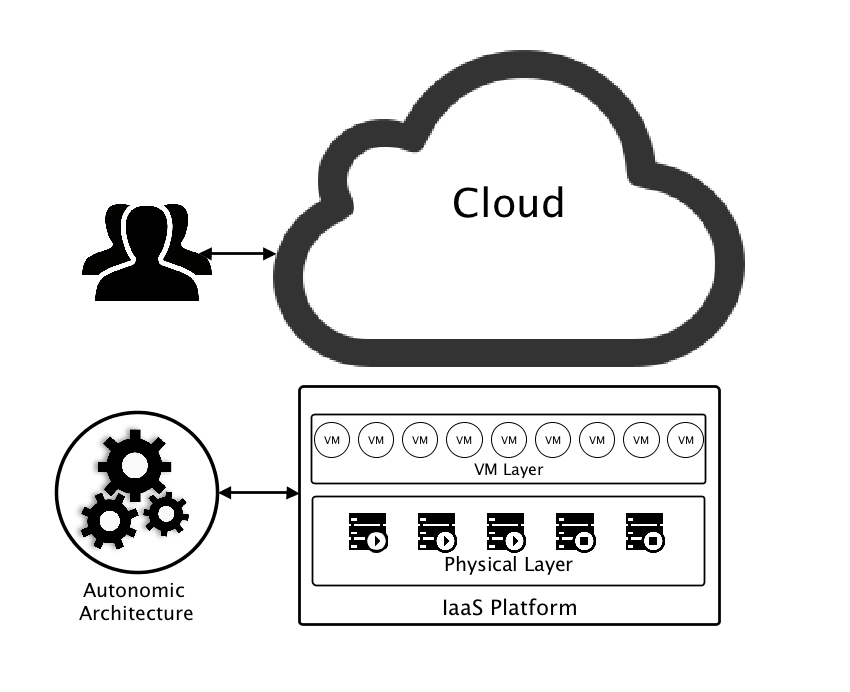
\includegraphics[scale=.32]{images/proposta.png}
	 \vspace{-8mm}
     \caption{Arquitetura Autonômica Aplicada à Computação em Nuvem}
   \end{figure}
% \end{block}
}


% % % % % % % % % % % % % % % % % % % % % %
% \section{Estudo de Caso}
% % % % % % % % % % % % % % % % % % % % % %
% \frame
% {
% 	\begin{LARGE}\begin{center}
% 	\textbf{Estudo de Caso}
% 	\end{center}\end{LARGE}
% }

\frame
{
\frametitle{Estudo de Caso}
\begin{block}{Integração}
	Este mecanismo será desenvolvido na forma de um componente integrado ao projeto de implantação de \textit{IaaS}  \textbf{\textit{OpenStack}}.
\end{block}
% \vspace{-8mm}
   \begin{figure}[bhtp]
     \centering 
\includegraphics[scale=.15]{images/openstack-logo.png}
	 \vspace{-8mm}
     % \caption{Arquitetura Autonômica Aplicada à Computação em Nuvem}
   \end{figure}
% \end{block}
% \begin{block}{Características que motivaram a escolha do \textbf{\textit{OpenStack}}:}
% 	\begin{itemize}
% 		\item Arquitetura mostra-se interessante para aplicação da proposta - desacoplamento;
% 		\item API madura e desenvolvida sobre um conjunto de padrões (abertos) estabelecido e fortalecidos atualmente;
% 		\item Documentação e Comunidade são pontos fortes do projeto - apoio de diversas entidades e empresas;
% 		% \item Crescente interesse da comunidade científica - e.g. em testes no LHC/CERN;
% 		\item Projeto de Código Aberto em franco de desenvolvimento.
% 	\end{itemize}
% \end{block}
}


%%%%%%%%%%%%%%%%%%%%%%%%%%%%%%%%%%%%%%%%%%%%%%%%%%%%%%%%%%%%%%%%%%
%
% Considerações Finais
%
%%%%%%%%%%%%%%%%%%%%%%%%%%%%%%%%%%%%%%%%%%%%%%%%%%%%%%%%%%%%%%%%%%

\section{Considerações Finais}
% \frame
% {
% 	\begin{LARGE}\begin{center}
% 	\textbf{Considerações Finais}
% 	\end{center}\end{LARGE}
% }

\frame
{
\frametitle{Considerações Finais}
\begin{block}{Desafios a enfrentar suscitados pelos trabalhos relacionados:}
	\begin{itemize}
		\item Determinar \textbf{\textit{quando e quais VMs migrar}} conforme o estado do ambiente;
		\item Determinar \textbf{\textit{onde alocar}} essas VMs;
		\item Determinar a \textbf{sobrecarga/subutilização de um nodo físico};
		\item Determinar \textbf{\textit{quando e quais nodos físicos} }serão colocados ou retirados de estado de minimização de consumo de energia;
		\item Como \textit{\textbf{lidar com diferentes tipos de carga de trabalho e suas flutuações}};
		\item Como lidar com o \textit{custos da manipulação} da infraestrutura, de forma \textbf{a atender a SLA}.
	\end{itemize}
\end{block}

}



\frame
{
\frametitle{Considerações Finais}
	\begin{block}{O que se mostrou mais relevante}\footnotesize
 		\begin{itemize}
			\item Computação em Nuvem: \textit{potencial frente de pesquisa} quanto à eficiência no consumo de energia;
			\item Natureza complexa e dinâmica de suas cargas de trabalho: \textit{desafios quanto ao gerenciamento da infraestrutura};
			\item \textit{Computação Autonômica pode colaborar} com a Computação em Nuvem;
			\note{auto-gestão, otimização}
 	   \end{itemize}
	\end{block}
	\begin{block}{Resumo do que será buscado}\footnotesize
 		\begin{itemize}
			\item Desenvolvimento de uma arquitetura que atenda as demandas da Computação em Nuvem quanto a eficiência energética, através estratégias proveniente da Computação Autonômica;
			\item Integração ao projeto de infraestrutura em nuvem \textit{OpenStack};
			\item Colaborar com as frentes de trabalhos relacionados a Computação Verde.
 \end{itemize}
\end{block}
}



% \frame
% {
% \frametitle{Cronograma das Atividades}
% % \begin{block}{}
% 	\vspace{-3mm}
% 	\begin{table}[htbp]\tiny
% 	\begin{center}
% 	\rowcolors{1}{}{Cerulean!12}
% 	\begin{tabular}{|c|c|c|c|c|c|c|c|c|c|c|c|c|}
% 	\hline
% 	\rowcolor{Cerulean!40}
% 	\tiny \cellcolor{Cerulean!60}{\small Ativ.\textbackslash Mês} & {\small 03} & {\small 04} & {\small 05} & {\small 06} & \cellcolor{Cerulean!55}{\small 07} & {\small 08} & {\small 09} & 
% 	{\small 10} & {\small 11} & {\small 12} & \cellcolor{Gray!20}{\small 01} & \cellcolor{Gray!20} {\small 02}\\\hline\hline
% 	{\small A1} & \cellcolor{Green!40}\textbullet & \cellcolor{Green!40}\textbullet & \cellcolor{Green!40}\textbullet & \cellcolor{Green!40}\textbullet &  &  &  &  &  &  &  &  \\\hline
% 	{\small A2} &  &  & \cellcolor{Green!40}\textbullet & \cellcolor{Green!40}\textbullet & \cellcolor{Green!40}\textbullet &  &  &  &  &  &  &  \\\hline
% 	{\small A3} &  &  &  & \cellcolor{Green!40}\textbullet & \cellcolor{Green!40}\textbullet & \textbullet &  &  &  &  &  &  \\\hline
% 	{\small A4} &  &  & & & \cellcolor{Green!40}\textbullet &  & & &  &  &
% 	&  \\\hline
% 	{\small A5} &  &  &  &  &  & \textbullet & \textbullet & \textbullet &  &  &  &  \\\hline
% 	{\small A6} &  &  &  & &  &  & & \textbullet & \textbullet & & & \\\hline
% 	{\small A7} &  &  &  &  &  &  &  & \textbullet & \textbullet & \textbullet &  &  \\\hline
% 	{\small A8} &  &  &  &  &  &  &  &  & \textbullet & \textbullet & \textbullet & \textbullet \\\hline
% 	{\small A9} &  &  &  &  \cellcolor{Green!40}\textbullet & \cellcolor{Green!40}\textbullet & \textbullet &  &  &  & \textbullet & \textbullet & \textbullet \\\hline
% 	{\small A10} & \cellcolor{Green!40}\textbullet & \cellcolor{Green!40}\textbullet & \cellcolor{Green!40}\textbullet & \cellcolor{Green!40}\textbullet  & \cellcolor{Green!40}\textbullet & \textbullet & \textbullet & \textbullet & \textbullet & \textbullet & \textbullet & \textbullet \\\hline 
% 	{\small A11} &  &  &  &  &  &  &  &  &  &  &  & \textbullet \\\hline
% 	\end{tabular}
% 	\end{center}
% 	\end{table}
% 	% \end{block}
% 	\begin{columns}
% 	    \begin{column}{58mm}
% 		\vspace{-14mm}
% 	   	\begin{block}{\small Realizadas}\scriptsize
% 			\vspace{-1mm}
% 	   		\begin{enumerate} \itemsep1pt \parskip0pt \parsep0pt
% 	   			\item[A1.] Revisão bibliográfica;
% 	   			\item[A2.] Avaliação das tecnologias para implementação de ambientes em nuvem;
% 	   			\item[A3.] Avaliação das técnicas de gerenciamento de energia;
% 	   			\item[A4.] Seminário de andamento;
% 	   		\end{enumerate}
% 			\vspace{-1mm}
% 	   	\end{block}
% 	    \end{column}
% 	    \hspace{-1mm}
% 	    \begin{column}{58mm}
% 			\vspace{-4mm}
% 			\begin{block}{\small Futuras ou em Andamento}\scriptsize
% 				\vspace{-0.9mm}
% 				\begin{enumerate} \itemsep1pt \parskip0pt \parsep0pt
% 					\setcounter{enumi}{4}
% 					\item[A5.] Desenvolvimento de heurísticas e estratégias para gerenciamento de energia;
% 					\item[A6.] Estudo das tecnologias para coleta de informação e atuação sobre \textit{hw} de servidores;
% 					\item[A7.] Elaboração de um modelo arquitetural; 
% 					\item[A8.] Prototipação, Validação, Avaliação;
% 					\item[A9.] Escrita de artigos;
% 					\item[A10.] Escrita da dissertação;
% 					\item[A11.] Defesa da dissertação.
% 				\end{enumerate}
% 				\vspace{-1mm}
% 			\end{block} 
% 	    \end{column}
% 	\end{columns}
% }
% % \frame{
% % 
% % BELOGLAZOV, A. Energy-efficient management of virtual machines in data centers for cloud computing. 2013.
% % 
% % 
% % }


\frame
{
\frametitle{}
	% \begin{block}{O que está sendo feito}
% 		Este trabalho encontra-se na fase inicial onde estão sendo estudados os tópicos relacionados a Computação em Nuvem e suas tecnologias, bem como aqueles relacionados as Computação Autonômica.
% 	\end{block}
	
	\begin{block}{Agradecimento}

		Projeto PRONEX/FAPERGS/CNPq GREEN-GRID Computação de Alto Desempenho Sustentável.
	\end{block}
}








%%%%%%%%%%%%%%%%%%%%%%%%%%%%%%%%%%%%%%%%%%%%
% Último Slide
%%%%%%%%%%%%%%%%%%%%%%%%%%%%%%%%%%%%%%%%%%%%
\frame
{
	\pgfdeclareimage[height=1.5cm]{logo}{images/lups_oficial.png}
	\logo{\pgfuseimage{logo}}
	
	\logo{\vspace{3mm} \begin{large} \textbf{Obrigado!} \end{large}}
    \titlepage
}
\end{document}

